\begin{align}
(I-D^2)(u_t + u_x) +D^2u_x = 0, \label{eq:basic_2}
\end{align}
where $D=\partial_x$.
Then we are required to solve the following PDE,
\begin{align}
\left\{
\begin{array}{l}
u_t + u_x + S = 0, \\
\left(I-D^2 \right)S = D^3 u .
\end{array}
\right.
\end{align}
When the hybrid scheme is applied, the advection equation
\begin{align}
u_t + u_x = 0,
\label{eq:append_advec}
\end{align}
is solved with the finite volume method, 
and then the fractional step method is applied to
the following equation,
\begin{align*}
u_t + S = 0.
\end{align*}

If we use the centered difference approximation of $O(\Delta x^2)$
accuracy, and the four-stage Runge-Kutta scheme for time stepping,
then we have,
\begin{align*}
U_1 &:= u^n \\
U_2 &:= u^n - \frac{\Delta t}{2}S_1, \quad  \textrm{where}\quad 
(I-D^2)S_1 = D^3 U_1, \\
U_3 &:= u^n - \frac{\Delta t}{2}S_2, \quad  \textrm{where}\quad
(I-D^2)S_2 = D^3 U_2, \\
U_4 &:= u^n - \Delta tS_3, \quad  \textrm{where}\quad
(I-D^2)S_3 = D^3 U_3, \\
u^{n+1} & = u^n -\frac{\Delta t}{6} \left[
S_1 + 2S_2 + 2S_3 + S_4
\right],  \quad  \textrm{where}\quad
(I-D^2)S_4 = D^3 U_4.
\end{align*}
For each step, $S_i$'s are computed from
\begin{align*}
& (S_i)_j - \frac{(S_i)_{j+1}-2(S_i)_j+(S_i)_{j-1}}{\Delta x^2} = 
\frac{u_{j+2} - 2u_{j+1} +2u_{j-1} -u_{j-2}}{2\Delta x^3}.
\end{align*}
In order to investigate the stability with von Neumann analysis,
replace $u_j= e^{i\xi j \Delta x}$ and  $(S_1)_j= \beta e^{i\xi j \Delta x}$. 
Simplification gives
\begin{align*}
&\beta \left( 1 - \frac{-2+2\cos(\xi \Delta x) }{\Delta x^2} \right) = 
\frac{\sin(2\xi \Delta x) - 2 \sin(\xi \Delta x)}{\Delta x^3} i, \\
& \beta = \frac{ -2\sin(\xi \Delta x)(1-  \cos(\xi \Delta x)) }
                     { \Delta x^3 +2\Delta x(1-\cos(\xi \Delta x))} i.
\end{align*}
Note that $\beta$ is a purely imaginary number.
If we replace the four-stage Runge-Kutta scheme with
$u_j= e^{i\xi j \Delta x}$ and  $(S_1)_j= \beta e^{i\xi j \Delta x}$, then we have
\begin{align*}
&S_1 = \beta e^{i\xi j \Delta x} ,
 \quad U_2 = \left(1-\frac{\Delta t\beta}{2} \right) e^{i\xi j \Delta x}\\
&S_2 = \beta \left(1-\frac{\Delta t\beta}{2} \right) e^{i\xi j \Delta x} ,
 \quad U_3 = \left(1- \frac{\Delta t\beta}{2}+\frac{(\Delta t\beta)^2}{4} \right) e^{i\xi j \Delta x}\\
&S_3 =  \beta\left(1- \frac{\Delta t\beta}{2}+\frac{(\Delta t\beta)^2}{4} \right)  e^{i\xi j \Delta x} , \\
& U_4 = \left(1-\Delta t\beta
+ \frac{(\Delta t\beta)^2}{2}-\frac{(\Delta t\beta)^3}{4} \right) e^{i\xi j \Delta x},\\
&S_4 = \beta \left(1-\Delta t\beta
+ \frac{(\Delta t\beta)^2}{2}-\frac{(\Delta t\beta)^3}{4} \right) e^{i\xi j \Delta x}.
\end{align*}
Thus the growth factor $g(\xi)$ is
\begin{align*}
g(\xi)= & 1-\frac{\Delta t}{6}\bigg[ \beta + 
2 \beta \left(1-\frac{\Delta t\beta}{2} \right) +
2 \beta\left(1- \frac{\Delta t\beta}{2}+\frac{(\Delta t\beta)^2}{4} \right) \\ 
&+ \beta \left(1-\Delta t\beta
+ \frac{(\Delta t\beta)^2}{2}-\frac{(\Delta t\beta)^3}{4} \right)
\bigg] \\
= & 1-\frac{1}{6}\left(
6\Delta t\beta -3(\Delta t\beta)^2 +(\Delta t\beta)^3-\frac{(\Delta t\beta)^4}{4}
\right).
\end{align*}
Since $\beta$ is an imaginary number,
let $\Delta t\beta= \gamma i$ for some real $\gamma$, and then we have
\begin{align*}
g(\gamma) & = 1-
\frac{1}{2}\gamma^2 +\frac{\gamma^4}{24} + \left(\frac{\gamma^3}{6} -\gamma \right)i \\
|g(\gamma)|^2 & = 1 + \frac{1}{4}\gamma^4 + \frac{\gamma^8}{24^2} -\gamma^2 + \frac{\gamma^4}{12}
-\frac{\gamma^6}{24} + \gamma^2 + \frac{\gamma^6}{36} -\frac{\gamma^4}{3} \\
& = 1 -\frac{1}{72}\gamma^6 + \frac{1}{576}\gamma^8.
\end{align*}
If $|\gamma|<2\sqrt{2}$, then $|g(\gamma)|<1$. 
The sufficient condition for stability is 
\begin{align}
\left| \frac{\Delta t}{\Delta x} \cdot \frac{ \sin(\xi \Delta x)(1-  \cos(\xi \Delta x)) }
                     { \Delta x^2 +2(1-\cos(\xi \Delta x))} \right| < \sqrt{2}, 
                     \quad \textrm{for~} \forall \xi \Delta x.
\end{align}
For small $\Delta x$, this condition approximately reduces to
\[
\frac{\Delta t}{\Delta x} < 2\sqrt{2}.
\]
The CFL condition for the advection equation
(\ref{eq:append_advec}) is a sufficient condition. 
Therefore, if the CFL condition is satisfied in the advection equation,
the fractional step is always stable with the suggested numerical scheme. 
\begin{align}
\left| \frac{\Delta t}{\Delta x} \cdot \frac{ \sin(\xi \Delta x)(1-  \cos(\xi \Delta x)) }
                     { \Delta x^2 +2(1-\cos(\xi \Delta x))} \right| < \sqrt{2}, 
                     \quad \textrm{for~} \forall \xi \Delta x.
\end{align}
For small $\Delta x$, this condition approximately reduces to

\section{Comparison of the Boussinesq equations}
\label{append:a}

A class of the Boussinesq-type equations can be written 
in the following form,
\begin{flalign}
& (H)_t + (Hu)_x = 0, \\
& (Hu)_t + \left( Hu^2 + \frac{gH²}{2} \right)_x + gHh_x + \psi = 0,
\end{flalign}
where $\psi$ represents dispersion terms.
If 
\begin{flalign}
\psi = \frac{Hh^2}{6} u_{xxt} - \frac{Hh}{2} (hu)_{xxt},
\label{eq:peregrine_disp}
\end{flalign}
then these are called 
the Peregrine's equations.

We claim that the Boussinesq equations 
by \citet{schaffer1993boussinesq}
can be approximately reduced to the Peregrine's form when $B=0$.
Since $H=h+\eta$, the dispersion terms of Sch{\"a}ffer and Madsen
with $B=0$, can be written as, 
\begin{flalign}
\psi = & \frac{1}{6}h^3 \left(\frac{Hu}{h} \right)_{xxt}
- \frac{1}{2}h^2 (Hu)_{xxt} \nonumber \\
= & \frac{1}{6}h^3 u_{xxt}
+ \frac{1}{6}h^3 \left( \frac{\eta u}{h} \right)_{xxt}
- \frac{1}{2}h^2 (hu)_{xxt} - \frac{1}{2}h^2 (\eta u)_{xxt} \nonumber \\
= & \frac{H h^2}{6} u_{xxt} - \frac{H h}{2} (hu)_{xxt} \nonumber \\
&- \frac{\eta h^2}{6} u_{xxt}
+ \frac{h^3}{6} \left( \frac{\eta u}{h} \right)_{xxt}
+ \frac{\eta h}{2} (hu)_{xxt}
- \frac{h^2}{2} (\eta u)_{xxt} \label{eq:append_schaffer_disp1} \\
= & \frac{H h^2}{6} u_{xxt} - \frac{H h}{2} (hu)_{xxt}
+ \mathcal{O}(\epsilon). \nonumber
\end{flalign}
Because the last four terms in (\ref{eq:append_schaffer_disp1})
are $\mathcal{O}(\epsilon$),
the dispersion terms of Sch{\"a}ffer and Madsen are approximately same as
the Peregrine's. 
However, due to the higher order terms in (\ref{eq:append_schaffer_disp1}),
Sch{\"a}ffer and Madsen's wave model has lower peak 
near the wave break
than the Peregrine's model. 

Now we will study the connection between 
Sch{\"a}ffer and Madsen's equations 
and Serre's equations. 
Use $H=h+\eta$ and $\eta_t = H_t = -(Hu)_x$,
and assume $\eta_{xx}$ is small. 
The dispersion terms of Sch{\"a}ffer and Madsen 
can be rewritten in a different form, 
\begin{flalign*}
\psi = & \frac{1}{6}h^3 \left(\frac{Hu}{h} \right)_{xxt}
- \frac{1}{2}h^2 (Hu)_{xxt} \\
= & - Hh h_xu_{xt} -\frac{1}{3} H h^2 u_{xxt}- H h \eta_xu_{xt} \\
& - \frac{1}{6} Hh \eta u_{xxt} 
+ \frac{1}{6} h \eta^2 u_{xxt} + h \eta (h+\eta)_x u_{xt} 
+ \frac{1}{6} h^3 \left( \frac{\eta u}{h} \right)_{xxt}
\end{flalign*}
Meanwhile
\begin{flalign*}
\left( \frac{\eta u}{h} \right)_{xxt} 
= & -\frac{2 h_x}{h^2}\eta u_{xt} 
+ \frac{2}{h} \eta_x u_{xt}
+ \frac{1}{h} \eta u_{xxt} 
+ \frac{2 h_x}{h^2} (Hu)_x u_{x} \\
&- \frac{2}{h} (Hu)_{xx} u_x 
- \frac{1}{h} (Hu)_x u_{xx}.
\end{flalign*}
Therefore $\psi$ reduces to 
\begin{flalign*}
\psi 
= & Hh\eta_xu_{xt} + \left( \frac{2}{3} h_x \eta  
- \frac{2}{3} h \eta_x  \right) hu_{xt} \\
& + \frac{1}{6} h^3 \left(\frac{2 h_x}{h^2} (Hu)_x u_{x}
- \frac{2}{h} (Hu)_{xx} u_x 
- \frac{1}{h} (Hu)_x u_{xx}  \right)  \\
= & - Hh h_xu_{xt} -\frac{1}{3} H h^2 u_{xxt}
+ \left( \frac{2}{3} h_x \eta  
- \frac{2}{3} h \eta_x  \right) hu_{xt} \\
& + \frac{1}{6} h^3 \left(\frac{2 h_x}{h^2} (Hu)_x u_{x}
- \frac{2}{h} (Hu)_{xx} u_x 
- \frac{1}{h} (Hu)_x u_{xx}  \right)
\end{flalign*}
Now consider the last term 
\begin{flalign*}
 & \frac{1}{6} h^3 \left(\frac{2 h_x}{h^2} (Hu)_x u_{x}
- \frac{2}{h} (Hu)_{xx} u_x 
- \frac{1}{h} (Hu)_x u_{xx}  \right) \\
= & \frac{1}{3} h \left( h_x (Hu)_x u_{x}
- h (Hu)_{xx} u_x 
- \frac{h}{2} (Hu)_x u_{xx}  \right) \\
= & \frac{1}{3} h \left( h_x \left( H_xu + Hu_x \right) u_{x}
- h \left( 2H_xu_x + Hu_{xx} \right) u_x 
- \frac{h}{2} (H_xu + Hu_x) u_{xx}  \right) \\
= & \frac{1}{3} h \left( h_x H (u_x)^2 
- 2H_x h (u_x)^2 - H h u_x u_{xx} 
- \frac{h}{2} H_x u u_{xx} - \frac{h}{2} H u_x u_{xx} \right) \\
= & \frac{1}{3} h \left( \left( h_x H - 2H_x h \right) (u_x)^2 
- \frac{3 H h}{2} u_x u_{xx} 
- \frac{h}{2} H_x u u_{xx} \right)
\end{flalign*}
If we rearrange (\ref{eq:madsen_new_disp_x}) and
assume that $h_x\eta$, $h_{xx}$ and $\eta_{xx}$ are small,
then 
the Madsen's dispersion terms can be written as
\begin{flalign*}
\psi 
\approx & - Hh h_xu_{xt} -\frac{Hh^2}{3} u_{xxt}- H h \eta_xu_{xt}
- \frac{1}{6} Hh \eta u_{xxt} 
+ \frac{1}{6} h^3 \left( \frac{\eta u}{h} \right)_{xxt}.
\end{flalign*}
Since $\eta_t = -(Hu)_x$, we have
\begin{flalign*}
\left( \frac{\eta u}{h} \right)_{xxt} 
\approx & \frac{2 \eta_x}{h} u_{xt}
+ \frac{\eta}{h} u_{xxt}  &+ \frac{2 h_x}{h^2} (Hu)_x u_{x}
- \frac{2}{h} (Hu)_{xx} u_x 
- \frac{1}{h} (Hu)_x u_{xx}.
\end{flalign*}
Plugging in and dropping small terms yields to 
\begin{flalign}
\psi 
\approx & - Hh h_xu_{xt} -\frac{Hh^2}{3} u_{xxt}- H h \eta_xu_{xt} 
- \frac{1}{6} Hh \eta u_{xxt} \nonumber \\
& +\frac{h^2\eta_x}{3} u_{xt}
+ \frac{h^2\eta}{6} u_{xxt} + \frac{h h_x}{3} (Hu)_x u_{x}
- \frac{h^2}{3} (Hu)_{xx} u_x 
- \frac{h^2}{6} (Hu)_x u_{xx} \nonumber \\
\approx & - Hh h_xu_{xt} -\frac{Hh^2}{3} u_{xxt}- H h \eta_xu_{xt} \nonumber \\
& +\frac{h^2\eta_x}{3} u_{xt}
 + \frac{h h_x}{3} (Hu)_x u_{x}
- \frac{h^2}{3} (Hu)_{xx} u_x 
- \frac{h^2}{6} (Hu)_x u_{xx}. \label{eq:madsen_disp_v3}
\end{flalign}
%\marginpar{\small I am not sure how to conclude the relation between Boussinesq and Serre.}

The Serre's equations of \citep{su1969korteweg}
has the following dispersion terms,
\begin{flalign}
\psi= &-Hhh_xu_{xt} - \frac{Hh^2}{3}u_{xxt}
- Hh\eta_xu_{xt} \nonumber \\
& - \frac{2}{3} Hh\eta u_{xxt}
+ \frac{Hh^2}{3}\left[ (u_x)^2-uu_{xx} \right]_x.
\label{eq:serre_disp}
\end{flalign}
It is observed that (\ref{eq:madsen_disp_v3}) and (\ref{eq:serre_disp}) share common terms.
As shown in Figure \ref{fig:bim_boussclaw_fun}
numerical results also show that Sch{\"a}ffer and Madsen's 
model is more similar to Serre's equations than Peregrine's equations.


Figure \ref{fig:bim_breaking} shows
the numerical results from the BIM model at $t=17$, $18$ and  $18.6$.
In the BIM results a vertical front is observed at $x=4.02$ and $t=18.6$
with the maximum wave amplitude $A=0.414$, and this shows similarity with 
the analysis of \citet{titov1995modeling}
on the wave breaking point.

%\begin{figure}[!htb]
%\centering
%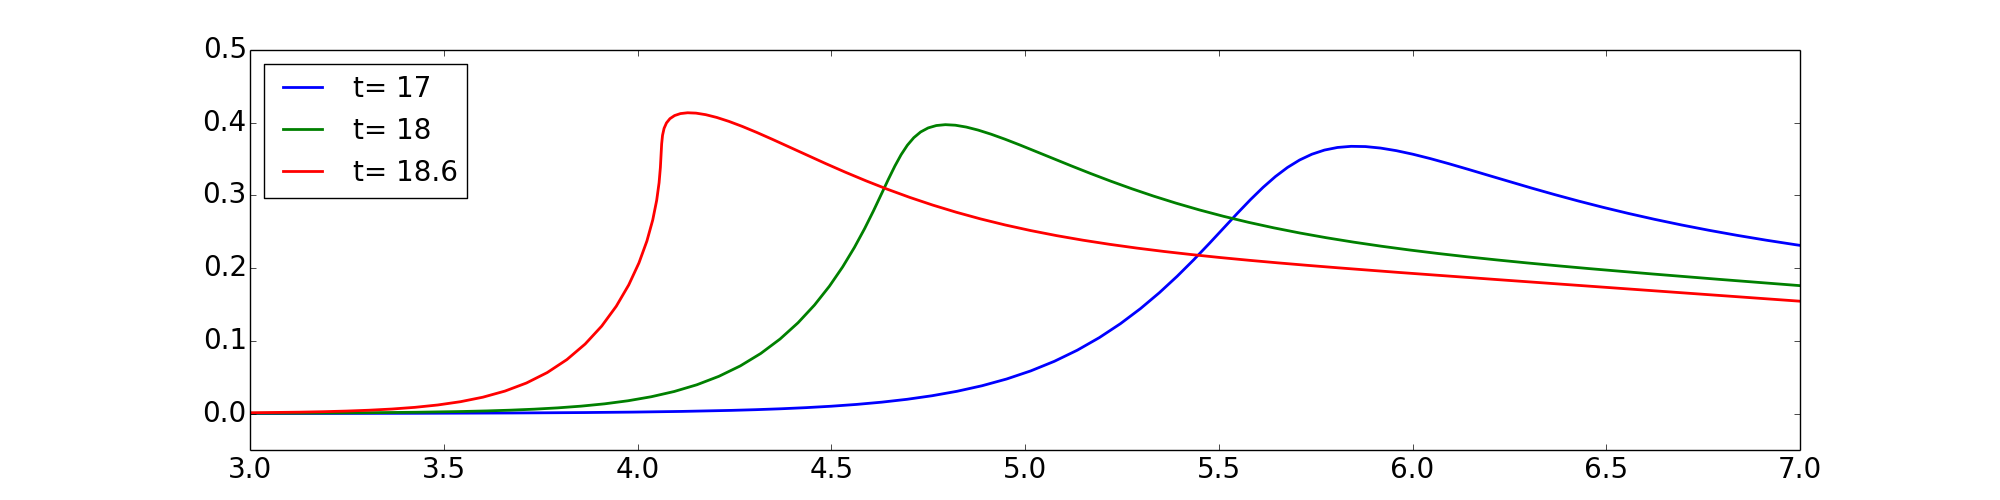
\includegraphics[width=\textwidth]{_fig/bim_n7_time_series.png}
%\caption{Computational results from BIM of a wave with $A/h=0.28$ on a slope of $1:19.85$.A vertical front is observed at $t=18.6$. }
%\label{fig:bim_breaking}
%\end{figure}
In Figure \ref{fig:sw_timeseries}, 
computations of the shallow water equations
(present model without the second fractional step) 
display a premature bore formation which checks the
amplification during the subsequent shoaling. 
As a consequence the amplitude 
in the shallow water equations simulation 
is markedly smaller than that of the 
potential flow model when the latter indicates breaking.




Boussinesq-type equations include non-hydrotstic pressure in an approximate way
treat short waves more accurately
than the shallow water equations. 
The Boussinesq-type wave models have been derived 
on the assumption that 
$\mathcal{O}(\epsilon)$ and $\mathcal{O}(\mu)$ terms
are small, where $\epsilon$ and $\mu$ 
denote the ratio of wave amplitude to depth
and the ratio of depth to wavelength respectively. 
Various models have been suggested,
and the papers of \citet{peregrine1967long},
\citet{madsen1992new}, \citet{nwogu1993alternative},
\citet{lynett2002modeling},
and \citet{wei1995time}
are representative examples. 
Assuming $\frac{1}{H}\int_{-h}^{\epsilon \eta} u^2 dz = \bar{u}^2$,
The vertically integrated wave energy densities for the NLSW 
and Boussinesq equations are $e_0$ and $e_0+e_1$, respectively, where
\begin{flalign}
& e_0 = \frac{1}{2}\left( g\eta^2 + H\bar{u}^2 \right), \label{eq:energy_e0} \\
& e_1 = \frac{1}{6}H^3\bar{u}_x^2
+ \frac{1}{2}H^2h_x\bar{u}\bar{u}_x + \frac{1}{2}Hh_x^2\bar{u}^2.
\label{eq:energy_e1}
\end{flalign}
Details are given in \citet{madsen1997surf} 
and in \ref{append:energy}. When the densities are integrated over the length of the numeric wave tank  we obtain the corresponding total energies (per width), 
denoted as $E_0$ and $E_1$.

The choice of the threshold could be identified as here, 
based on numerical models, 
or alternatively be determined based on the experiments.
The threshold can vary case by case as noted
by \cite{lynett2006nearshore} and \cite{matsuyama2007study} 
for example.\todo{Geir: I do not understand this} 
